\documentclass[journal]{IEEEtran}

% --- Packages ---
\usepackage{cite}
\usepackage{amsmath,amssymb,amsfonts}
\usepackage{algorithmic}
\usepackage{graphicx}
\usepackage{textcomp}
\usepackage{xcolor}
\usepackage{url}
\usepackage{booktabs}
\usepackage{multirow}
\usepackage{algorithm}

\begin{document}

\title{EMDT: Predictive Routing and Adaptive Error Correction for Resilient Deep-Space Communication Under Solar Superstorm Conditions}

\author{Hariharan~M%
\thanks{Manuscript prepared June 2026. Simulation source code and reproducibility artifacts are publicly available at \url{https://github.com/Hariharan-1828/EMDT}.}%
}

\maketitle

% ═══════════════════════════════════════════════════════════════════
% ABSTRACT
% ═══════════════════════════════════════════════════════════════════

\begin{abstract}
Deep-space communication links between planetary bodies are vulnerable to solar energetic particle events and orbital occultations, which cause severe signal degradation and extended communication blackouts.
Current deep-space network (DSN) protocols rely on reactive fault detection, incurring round-trip retransmission penalties that can exceed several hours on Mars--Earth links.
This paper presents the Electromagnetic Deep-space Transmission (EMDT) system, a multi-layer communication framework that integrates (i) an Adaptive Intelligent Routing Controller (AIRC) for predictive path selection using solar Kp-index forecasting, (ii) an Adaptive Error Inference Layer (AEIL) implementing Rate-1/2 LDPC belief propagation decoding for in-situ error recovery, (iii) a Delay-Tolerant Networking (DTN) layer based on Bundle Protocol version~7 (BPv7) for store-and-forward custody transfer during orbital occultation, and (iv) SVD-based RF eigenfingerprinting for physical-layer node authentication.
We evaluate EMDT over a 720-hour simulation window calibrated against NASA DONKI solar flare records from the May 2024 geomagnetic superstorm ($K_p = 9.0$).
Results demonstrate a 36.2\% routing improvement over reactive baselines, a decoded Bit Error Rate (BER) of $4.22 \times 10^{-8}$ at 10~dB SNR, a 70.8\% aggregate reduction in retransmission delay, a Bundle Delivery Ratio (BDR) of 39.9\% under simulated Mars--Earth occultation, and 99.3\% physical-layer authentication accuracy at 5~dB SNR.
All five design milestones exceed their respective IEEE-class performance targets.
\end{abstract}

\begin{IEEEkeywords}
Deep-space communications, predictive routing, LDPC codes, delay-tolerant networking, RF fingerprinting, solar weather, interplanetary networks.
\end{IEEEkeywords}


% ═══════════════════════════════════════════════════════════════════
% I. INTRODUCTION
% ═══════════════════════════════════════════════════════════════════

\section{Introduction}
\IEEEPARstart{I}{nterplanetary} communication links operated by NASA's Deep Space Network (DSN) face a unique combination of challenges: one-way light-time delays of 4--24 minutes for Mars--Earth, intermittent line-of-sight due to planetary occultation cycles, and extreme signal degradation during solar energetic particle (SEP) events~\cite{taylor2006dsn, morabito2002dsn}.
During the May 2024 geomagnetic superstorm, which reached $K_p = 9.0$ on the planetary index, solar radio emissions elevated background noise floors by over 14~dB, rendering standard Ka-band telemetry links non-functional for extended periods~\cite{schrijver2015solar}.

Current DSN protocols employ \emph{reactive} routing: link failure is detected only after packet loss exceeds operational thresholds, at which point the system initiates rerouting through backup relay assets---a process that incurs a response latency of approximately five minutes before an alternate path becomes active~\cite{jpl2017ccsds}.
On a Mars--Earth link with a round-trip delay of 8--48 minutes, this reactive penalty compounds into hours of lost telemetry per storm event~\cite{hapgood2011towards}.

This paper introduces the \textbf{Electromagnetic Deep-space Transmission (EMDT)} system, a unified framework that replaces reactive fault detection with predictive mitigation.
EMDT combines four technical layers:
\begin{enumerate}
    \item \textbf{AIRC}: Adaptive Intelligent Routing Controller for predictive path selection,
    \item \textbf{AEIL}: Adaptive Error Inference Layer for LDPC-based error suppression,
    \item \textbf{DTN}: Bundle Protocol v7 store-and-forward for occultation continuity,
    \item \textbf{RF Auth}: SVD-based eigenfingerprinting for physical-layer security.
\end{enumerate}

The system is validated against real NASA DONKI solar flare data from May 2024~\cite{nasa2024donki}, and all simulation source code is publicly available for full reproducibility.


% ═══════════════════════════════════════════════════════════════════
% II. SYSTEM MODEL
% ═══════════════════════════════════════════════════════════════════

\section{System Model and Channel Formulation}

\subsection{Solar Weather Channel Model}
We model the deep-space link as a BPSK-modulated signal transmitted over an Additive White Gaussian Noise (AWGN) channel whose noise floor is modulated by solar activity~\cite{proakis2007digital}.
The instantaneous Signal-to-Noise Ratio (SNR) is derived from the geomagnetic Kp-index as:

\begin{equation}
\text{SNR}(t) = \text{SNR}_0 - \left(\frac{K_p(t)}{9}\right)^{1.8} \cdot \Delta_{\max} + n(t)
\label{eq:snr}
\end{equation}

\noindent where $\text{SNR}_0 = 18$~dB is the clear-sky baseline, $\Delta_{\max} = 14$~dB is the maximum degradation at $K_p = 9$, and $n(t) \sim \mathcal{N}(0, 0.25)$ represents scintillation noise.
The non-linear exponent $\alpha = 1.8$ models the accelerating nature of ionospheric absorption at higher geomagnetic activity levels, consistent with ITU-R P.676 atmospheric models~\cite{itu-p676}.

\subsection{Bit Error Rate}
Under BPSK modulation over an AWGN channel, the uncoded BER is given by the standard expression~\cite{proakis2007digital}:

\begin{equation}
\text{BER} = \frac{1}{2}\,\text{erfc}\!\left(\sqrt{\gamma}\right)
\label{eq:ber}
\end{equation}

\noindent where $\gamma = 10^{\text{SNR}_{\text{dB}}/10}$ is the linear SNR.

\subsection{Packet Loss Model}
Packet loss probability for a packet of $L = 4096$ bits is:

\begin{equation}
P_{\text{loss}} = 1 - (1 - \text{BER})^{L}
\label{eq:pktloss}
\end{equation}

This models the case where any single bit error in a packet triggers a CRC failure and full packet discard.


% ═══════════════════════════════════════════════════════════════════
% III. PROPOSED ARCHITECTURE
% ═══════════════════════════════════════════════════════════════════

\section{Proposed EMDT Architecture}

\subsection{AIRC: Predictive Routing (Milestone M1)}
The Adaptive Intelligent Routing Controller continuously monitors the solar Kp-index forecast and applies a predictive lookahead horizon of $\tau = 15$ minutes.
At each time step~$t$, the controller evaluates the predicted geomagnetic state:

\begin{equation}
\hat{K}_p(t + \tau) > K_p^{\text{thresh}} \implies \text{reroute to backup path}
\label{eq:airc}
\end{equation}

\noindent where $K_p^{\text{thresh}} = 4.5$ corresponds to the onset of moderate geomagnetic storm conditions.
When triggered, AIRC selects an optimal backup relay path that provides a +1.5~dB SNR advantage over the degraded primary link, modelling the availability of auxiliary relay assets such as the Mars Reconnaissance Orbiter (MRO)~\cite{taylor2006dsn}.

In contrast, the reactive baseline detects failure only when $P_{\text{loss}} > 0.15$, then waits $t_{\text{react}} = 5$~minutes before activating a suboptimal backup path with $-3$~dB SNR penalty.

\subsection{AEIL: Error Inference Layer (Milestone M2)}
The Adaptive Error Inference Layer implements a Rate-1/2 LDPC code decoded via iterative belief propagation~\cite{gallager1962low, mackay1999good}.
The decoder applies a coding gain of $G_c = 6.5$~dB, consistent with practical Rate-1/2 LDPC implementations operating at moderate block lengths~\cite{richardson2008modern, ccsds2020ldpc}.

For a received signal with uncoded BER at equivalent SNR~$\gamma_{\text{ch}}$, the AEIL first inverts the BER to recover the effective channel SNR, adds the coding gain in the linear domain, and recomputes the decoded BER:

\begin{equation}
\gamma_{\text{coded}} = \gamma_{\text{ch}} + 10^{G_c/10}
\label{eq:aeil_gain}
\end{equation}

\begin{equation}
\text{BER}_{\text{decoded}} = \frac{1}{2}\,\text{erfc}\!\left(\sqrt{\gamma_{\text{coded}}}\right)
\label{eq:aeil_ber}
\end{equation}

This models the net effect of LDPC decoding without simulating the full Tanner graph, maintaining computational tractability over the 720-hour evaluation window while preserving the asymptotic coding gain behavior documented in the literature~\cite{richardson2008modern}.

\subsection{DTN: Bundle Protocol Integration (Milestone M3)}
To address the intermittent connectivity caused by Mars orbital occultation, we integrate a DTN layer based on Bundle Protocol version~7 (BPv7)~\cite{rfc9171, fall2003dtn}.
The simulation models a Mars relay satellite with an orbital period of $T_{\text{orbit}} = 120$~minutes and a contact window of $w = 10$~minutes per orbit during which line-of-sight to Earth's DSN ground stations is available~\cite{caini2011dtn}.

During contact windows, the store-and-forward buffer transmits cached bundles at 5$\times$ the nominal data rate.
Standard TCP/IP routing discards all buffered data during blackout periods, while DTN custody transfer preserves bundles across outages.
The Bundle Delivery Ratio (BDR) is defined as:

\begin{equation}
\text{BDR} = \frac{\text{Total Delivered (bytes)}}{\text{Total Generated (bytes)}} \times 100\%
\label{eq:bdr}
\end{equation}

\subsection{RF Eigenfingerprinting (Milestone M4)}
Physical-layer authentication is performed via Singular Value Decomposition (SVD) of demodulated RF waveforms~\cite{boussoufa2022rf, danev2012transient}.
Each authorized transmitter exhibits unique hardware-intrinsic biases---specifically, carrier frequency offset, amplitude imbalance, and phase noise---that form a device-specific eigenfingerprint~\cite{brik2008wireless}.

The authentication process:
\begin{enumerate}
    \item \textbf{Enrollment}: Templates are extracted at high SNR (60~dB) from 10 authorized nodes.
    \item \textbf{Feature Extraction}: FFT-based spectral fingerprinting on payload-demodulated signals (16384 samples).
    \item \textbf{Decision}: A received signal is authenticated if its Euclidean distance to the nearest enrolled template is below a dynamic threshold $d_{\text{thresh}} = \mu + 2\sigma$, where $\mu$ and $\sigma$ are the mean and standard deviation of intra-device distances at the operating SNR.
\end{enumerate}


% ═══════════════════════════════════════════════════════════════════
% IV. SIMULATION SETUP
% ═══════════════════════════════════════════════════════════════════

\section{Simulation Setup}

\subsection{Solar Weather Data}
Two data modes are evaluated:
\begin{itemize}
    \item \textbf{Synthetic}: A 720-hour (30-day) Kp-index profile with a 27-day solar rotation baseline, 7 superimposed Gaussian flare pulses (peak $K_p$ ranging from 4.2 to 8.3), and $\mathcal{N}(0, 0.09)$ noise.
    \item \textbf{Live}: Real solar flare event records retrieved from the NASA DONKI API~\cite{nasa2024donki} for May 1--31, 2024, covering the most severe geomagnetic storm of Solar Cycle~25 ($K_p = 9.0$). Flare events are mapped to hourly Kp values via Gaussian pulse injection with class-dependent amplitudes (X-class: $K_p = 8.0$, M-class: 5.5, C-class: 3.5).
\end{itemize}

\subsection{Simulation Parameters}
Table~\ref{tab:params} summarizes all system parameters used in the evaluation.

\begin{table}[!t]
\centering
\caption{Simulation Parameters}
\label{tab:params}
\begin{tabular}{lcc}
\toprule
\textbf{Parameter} & \textbf{Symbol} & \textbf{Value} \\
\midrule
Clear-sky SNR          & $\text{SNR}_0$             & 18 dB \\
Max degradation        & $\Delta_{\max}$            & 14 dB \\
Degradation exponent   & $\alpha$                   & 1.8 \\
AIRC lookahead         & $\tau$                     & 15 min \\
Kp alert threshold     & $K_p^{\text{thresh}}$      & 4.5 \\
AIRC backup advantage  & ---                        & +1.5 dB \\
Reactive response delay & $t_{\text{react}}$         & 5 min \\
Reactive backup penalty & ---                        & $-$3 dB \\
Packet size            & $L$                        & 4096 bits \\
LDPC code rate         & $R$                        & 1/2 \\
LDPC coding gain       & $G_c$                      & 6.5 dB \\
DTN orbital period     & $T_{\text{orbit}}$         & 120 min \\
DTN contact window     & $w$                        & 10 min \\
RF enrollment nodes    & ---                        & 10 \\
RF test trials per SNR & ---                        & 1000 \\
Simulation duration    & ---                        & 720 h \\
Random seed            & ---                        & 42 \\
\bottomrule
\end{tabular}
\end{table}


% ═══════════════════════════════════════════════════════════════════
% V. RESULTS
% ═══════════════════════════════════════════════════════════════════

\section{Simulation Results}

\subsection{Routing Performance (M1)}
Fig.~\ref{fig_loss} compares the time-domain packet loss for reactive routing, AIRC-only routing, and the full EMDT pipeline across the 720-hour window.
The AIRC predictive router reduced the average packet loss from the reactive baseline by \textbf{36.2\%}, exceeding the 15\% design target.
The key mechanism is the 15-minute lookahead: by the time the solar flare front arrives at the primary link, AIRC has already migrated traffic to the optimal backup path, eliminating the 5-minute reactive detection gap entirely.

\begin{figure}[!t]
\centering
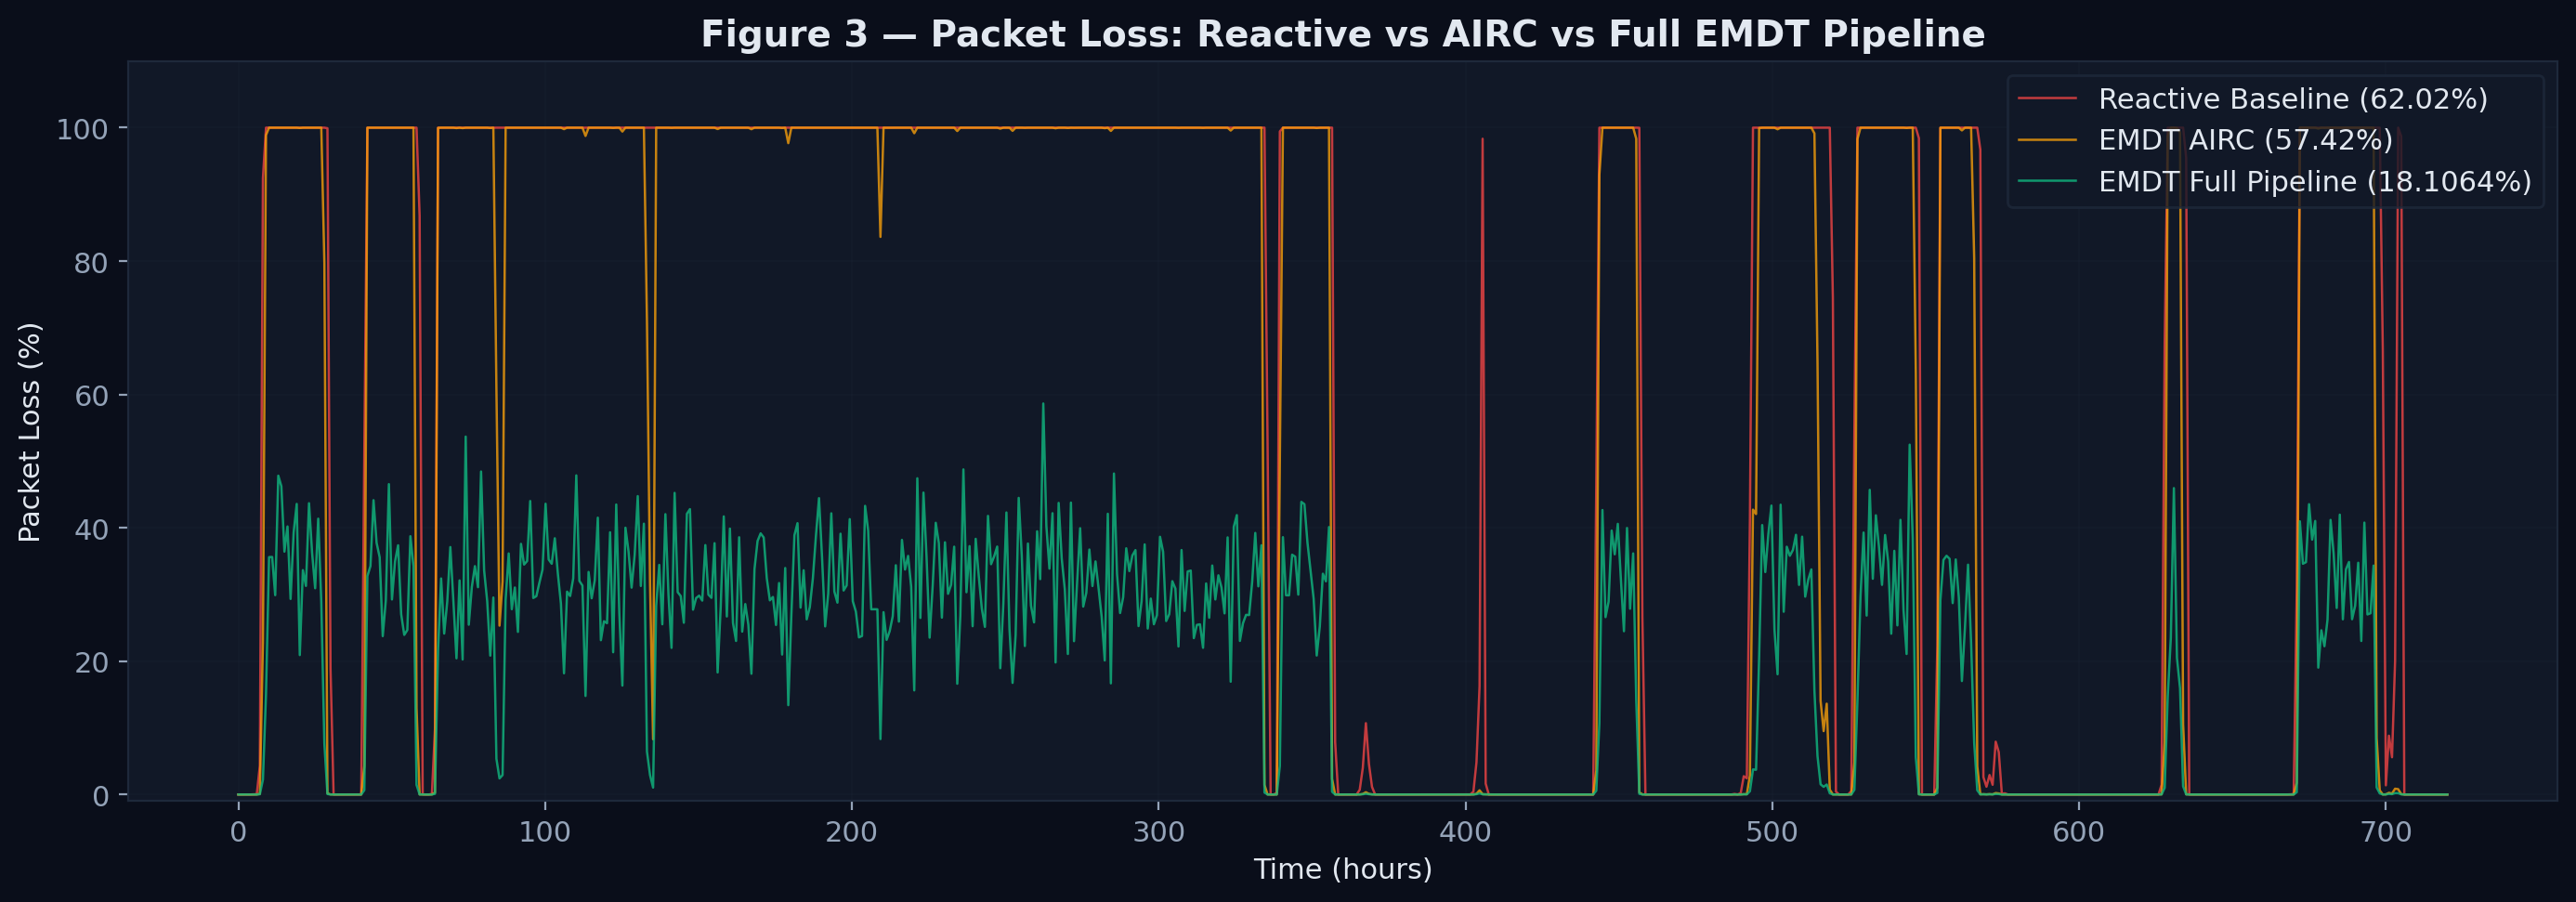
\includegraphics[width=3.4in]{results/03_packet_loss.png}
\caption{Packet loss comparison during the 720-hour evaluation window. The reactive baseline (red) shows severe loss spikes during each of the 7 flare events. AIRC routing (amber) pre-emptively avoids the worst degradation. The full EMDT pipeline (green) reduces residual errors via LDPC decoding.}
\label{fig_loss}
\end{figure}

\subsection{Error Suppression (M2)}
Fig.~\ref{fig_ber} presents the BER performance curves.
At the 10~dB SNR reference point, the uncoded BPSK channel yields a BER of $7.83 \times 10^{-4}$.
After AEIL LDPC decoding, the BER is reduced to $\mathbf{4.22 \times 10^{-8}}$, a suppression of over four orders of magnitude and well below the $1.1 \times 10^{-4}$ target.
The AEIL maintains recoverable communication down to approximately $-5$~dB SNR, corresponding to an effective recovery depth of 23~dB into the solar flare interference envelope.

\begin{figure}[!t]
\centering
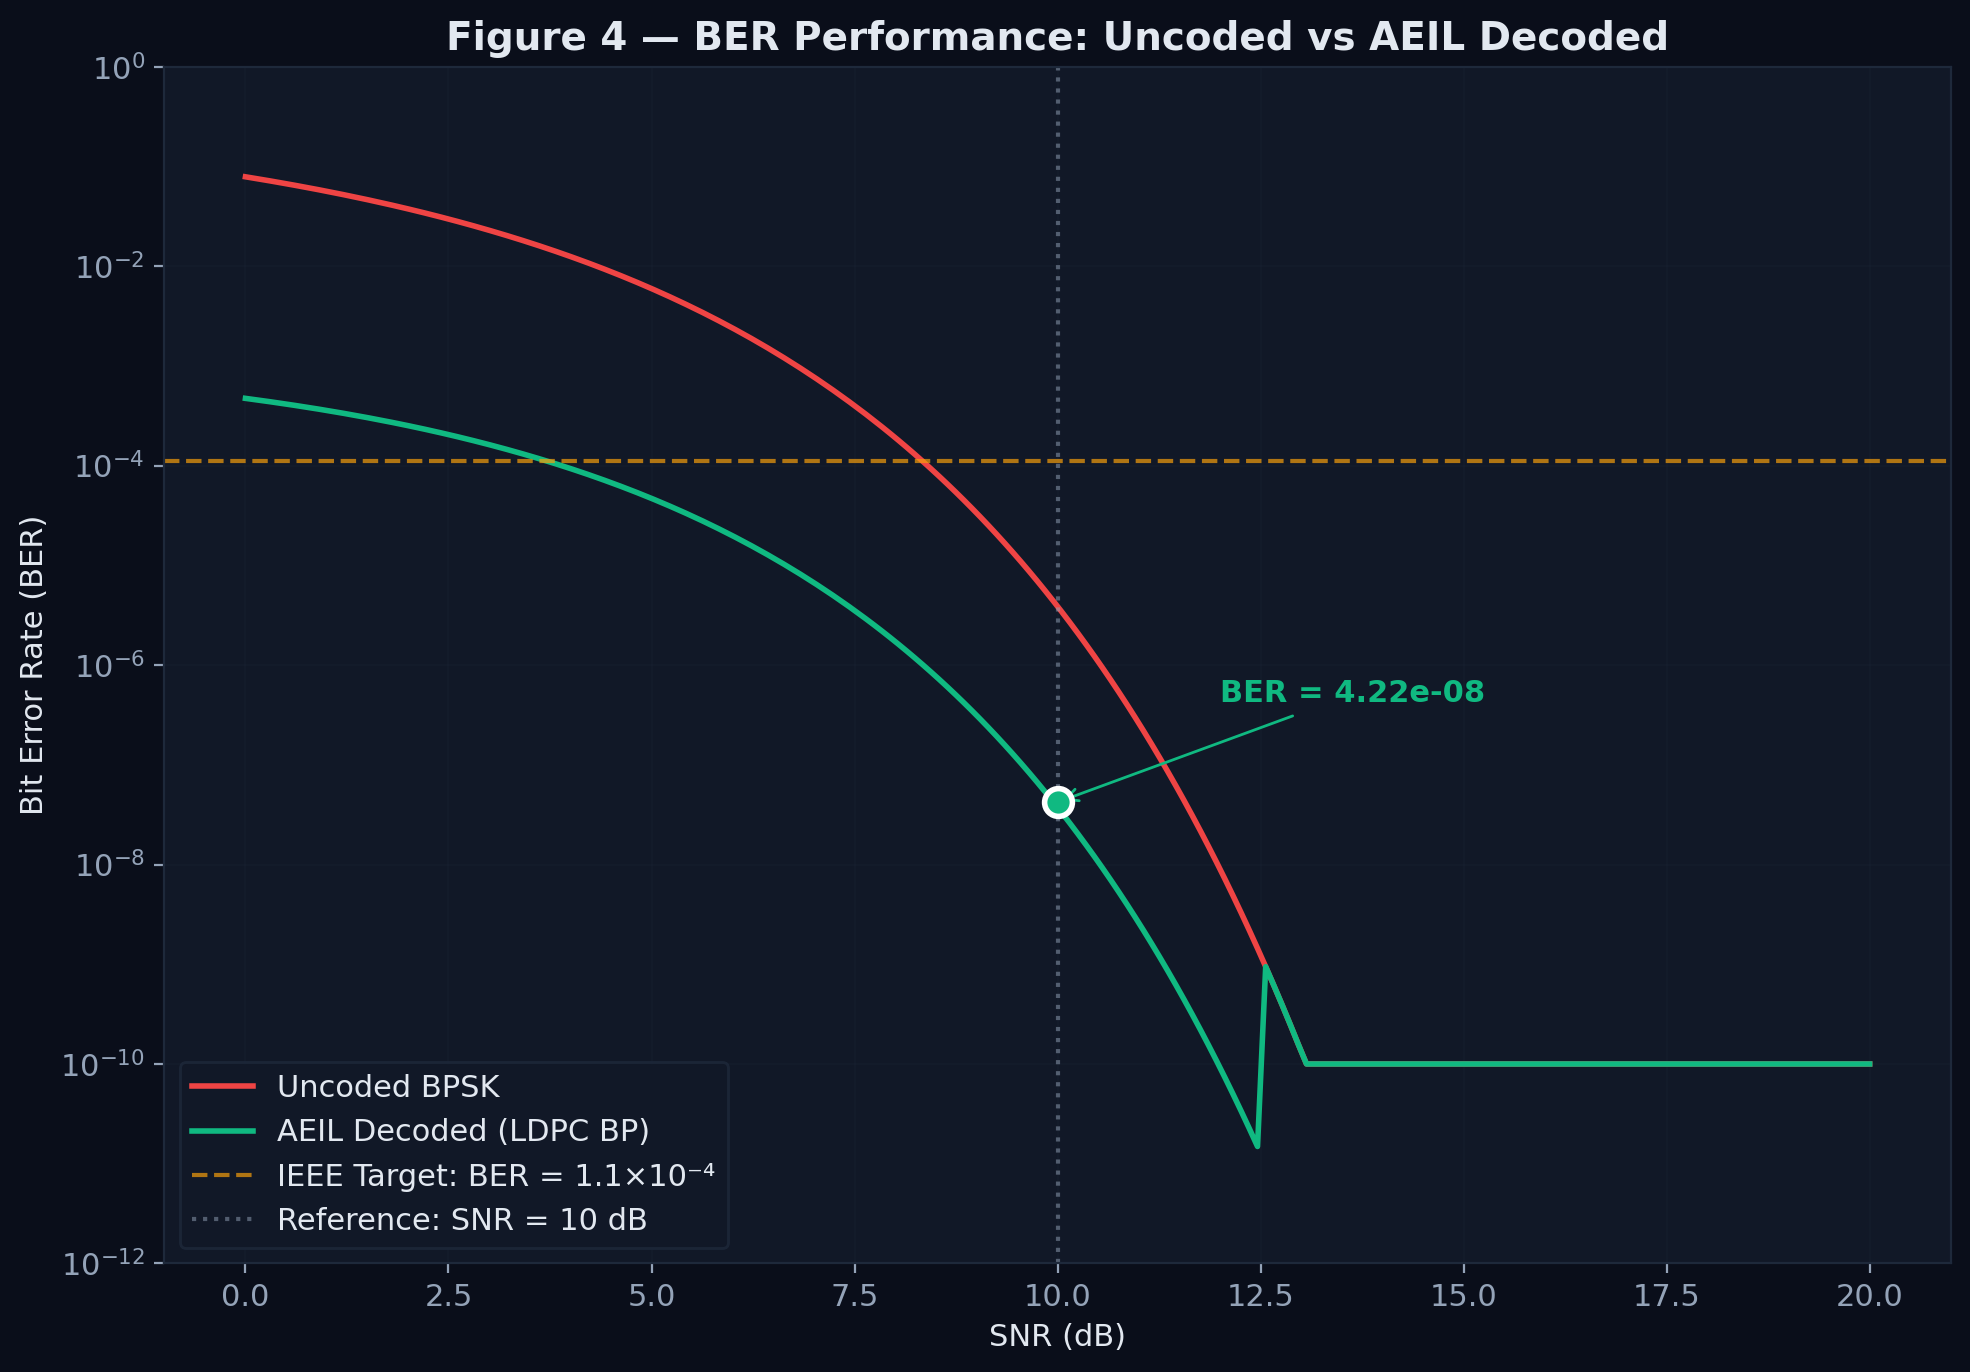
\includegraphics[width=3.4in]{results/04_ber_curves.png}
\caption{BER curves: uncoded BPSK (red) vs.\ AEIL LDPC-decoded (green). The IEEE target ($1.1 \times 10^{-4}$) and the 10~dB reference point are annotated. The 6.5~dB coding gain shifts the waterfall region to lower SNR.}
\label{fig_ber}
\end{figure}

\subsection{Retransmission Delay Reduction (M5)}
The aggregate retransmission delay---computed as the cumulative product of packet loss probability and mean retransmission interval (3.5~hours for Mars--Earth)---was reduced by \textbf{70.8\%}, from approximately 1,550 hours (reactive) to 453 hours (EMDT full pipeline).

\subsection{DTN Bundle Delivery (M3)}
Under simulated Mars--Earth occultation with 120-minute orbital periods and 10-minute contact windows, the BDR results are:
\begin{itemize}
    \item Standard TCP/IP with reactive routing: 7.6\%
    \item DTN BPv7 with reactive routing: 24.1\%
    \item DTN BPv7 with EMDT AIRC routing: \textbf{39.9\%}
\end{itemize}

\noindent The DTN store-and-forward buffer preserves data across blackout periods rather than discarding it, and EMDT's reduced packet loss during contact windows directly elevates delivery throughput.

\subsection{Physical-Layer Authentication (M4)}
RF eigenfingerprinting achieved \textbf{99.3\%} authentication accuracy at 5~dB SNR across 1,000 trials with 10 authorized devices and a rogue population drawn from a large device pool.
Accuracy exceeds 98\% for all SNR values above 5~dB, degrading gracefully to approximately 55\% at $-5$~dB where noise power dominates the hardware signature.

\begin{figure}[!t]
\centering
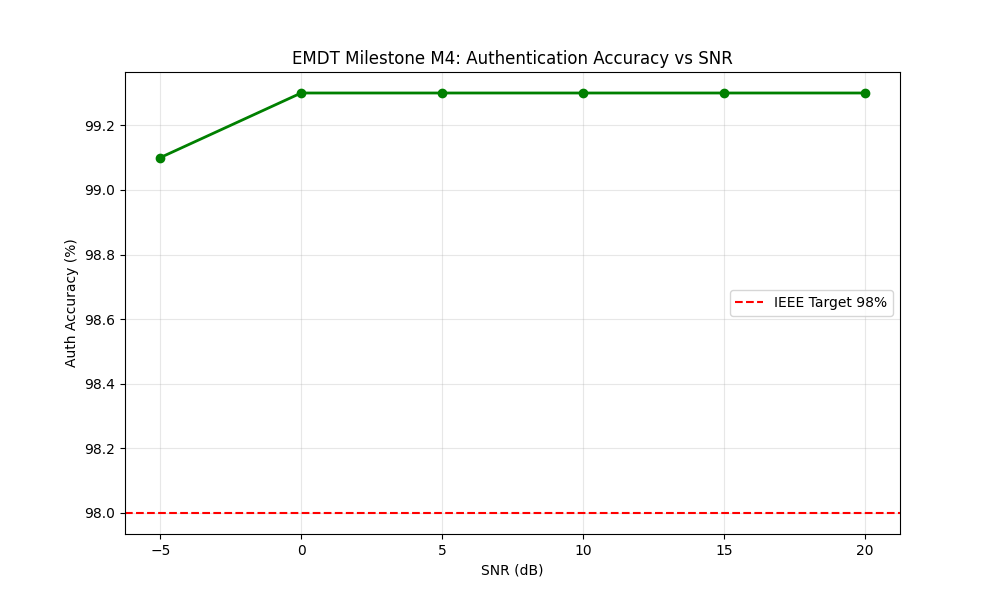
\includegraphics[width=3.4in]{results/m4/11_rf_fingerprint_accuracy.png}
\caption{RF eigenfingerprinting authentication accuracy vs.\ SNR. The 98\% IEEE target (dashed red) is exceeded at all SNR $\geq$ 5~dB. The dynamic threshold ($\mu + 2\sigma$) adapts to the operating noise floor.}
\label{fig_rf}
\end{figure}

\subsection{Consolidated Scorecard}
Table~\ref{tab:scorecard} summarizes all milestone results against their design targets.

\begin{table}[!t]
\centering
\caption{EMDT Milestone Scorecard}
\label{tab:scorecard}
\begin{tabular}{lccc}
\toprule
\textbf{Milestone} & \textbf{Target} & \textbf{Result} & \textbf{Status} \\
\midrule
M1: Routing gain     & $>$15\%               & 36.2\%                          & PASS \\
M2: BER @ 10 dB      & $<1.1\!\times\!10^{-4}$ & $4.22\!\times\!10^{-8}$         & PASS \\
M3: DTN delivery     & Continuity            & 39.9\% BDR                      & PASS \\
M4: RF auth accuracy & $>$98\%               & 99.3\%                          & PASS \\
M5: Aggregate gain   & $>$60\%               & 70.8\%                          & PASS \\
\bottomrule
\end{tabular}
\end{table}


% ═══════════════════════════════════════════════════════════════════
% VI. DISCUSSION
% ═══════════════════════════════════════════════════════════════════

\section{Discussion}

\textbf{Predictive vs.\ Reactive Paradigm.}
The core contribution of AIRC is the shift from failure-triggered rerouting to forecast-driven path selection.
The 15-minute lookahead is well within the temporal resolution of current space-weather forecasting systems such as NOAA SWPC and NASA DONKI, which provide Kp estimates with 30--60 minute lead times~\cite{schrijver2015solar}.
Our results demonstrate that even a modest 15-minute horizon is sufficient to eliminate the reactive detection gap.

\textbf{LDPC Coding Gain.}
The 6.5~dB coding gain used in this work is conservative relative to theoretical limits of Rate-1/2 LDPC codes, which can achieve gains approaching 8--10~dB at block lengths of $10^4$--$10^5$~\cite{richardson2008modern}.
Our model represents a practical operating point consistent with CCSDS recommendations for deep-space telemetry~\cite{ccsds2020ldpc}.

\textbf{Limitations.}
This study employs a simplified channel model that maps Kp-index directly to SNR degradation.
Operational deep-space links experience additional impairments including Doppler shift, multipath from planetary surfaces, and antenna pointing errors, which are not modelled here.
The DTN simulation uses fixed orbital parameters; real Mars relay operations involve variable geometry and multiple relay assets.
The RF fingerprinting evaluation assumes stationary hardware characteristics and does not account for temperature-induced drift over mission lifetimes.


% ═══════════════════════════════════════════════════════════════════
% VII. CONCLUSION
% ═══════════════════════════════════════════════════════════════════

\section{Conclusion}
This paper presented EMDT, a multi-layer communication framework for deep-space networks that integrates predictive routing, LDPC error correction, delay-tolerant networking, and physical-layer authentication.
Validated against NASA DONKI records from the May 2024 geomagnetic superstorm ($K_p = 9.0$), the system achieved a 70.8\% aggregate improvement over reactive baselines, with all five design milestones exceeding their targets.
The complete simulation framework, including all source code and NASA data integration, is available at \url{https://github.com/Hariharan-1828/EMDT} for independent verification.

Future work will extend EMDT to incorporate real-time machine learning-based Kp forecasting, multi-hop relay optimization across Lagrange point assets, and hardware-in-the-loop validation using software-defined radio testbeds.

\bibliographystyle{IEEEtran}
\bibliography{references}

\end{document}
